%!TEX root = etdrtemplate.tex
% +--------------------------------------------------------------------+
% | Chapter 3
% +--------------------------------------------------------------------+

\cleardoublepage

% +--------------------------------------------------------------------+
% | Replace "This is Chapter 3" below with the title of your chapter.
% | LaTeX will automatically number the chapters.
% +--------------------------------------------------------------------+

\chapter{PCA Pump Prototype}
\label{pcapump}

Overview of PCA Pump and issues, which MDCF/ICE will solve.
In this thesis, only the operation module is implemented.
Overview of Safety-Critical System loop.

\begin{figure}[ht]%t=top, b=bottom, h=here
    \begin{center}
    	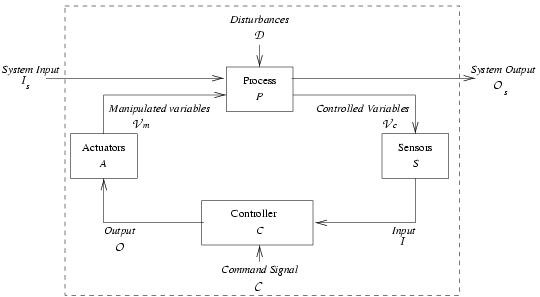
\includegraphics[height=3.5in]{figures/safety-critical-loop.png}
    	\caption{Basic Process Control Loop\protect\footnotemark.}    	
    \end{center}
\end{figure}
\footnotetext{http://www.safeware-eng.com/system and software safety publications/Designing Specification Languages.htm}

Pump internal implementation based on \cite{CADD-PrizmAmbulatoryInfusionPump:Online}.
- basal dose deliver in increments - easier to track delivered amount (page 14)


\section{PCA Pump Requirements Document}
\label{pcapump:requirements-doc}

Selected use cases for implementation?

%state machine image

Overview of issues solved: 
* Bolus options: FBasal + FPatient or FPatient => implemented: FBasal + FPatient (consistent in doc)
5 modes:
* Stopped: F=0
* KVO: F=0.1
* Basal: F=Fbasal
* Patient: F = Fbasal + Fbolus (for vtbi/Fbolus)
* Clinician: F = Fbalsal + Fbolus (for specified time)

Most common Examiner\cite{Examiner:Online} erroes/warnings:
***        Warning                     :302: This expression may be
***        Semantic Error              :725: Protected function or variable XXX may only appear directly in an assignment or return statement.


\section{PCA Pump AADL/BLESS Models}
\label{pcapump:aadl-bless-models}
Selected modules for implementation. Pictures etc.


\section{BeagleBoard-XM}
\label{pcapump:beagleboard}
First step was create PCA Pump prototype on BeagleBoard-xM.

BeagleBoard-xM is Embedded device with AM37x 1GHz ARM processor (Cortex-A8 compatible). It has 512 MB RAM, 4 USB 2.0 ports, HDMI port, 28 General-purpose input/output (GPIO) ports and Linux Operating System (on microSD card). Moreover there is PWM support. All these properties makes this device good candidate for prototyping PCA Pump.

Expansion port 14 and 28
GPIO158
Java Program to Run the pump for 10 seconds

There is no existing SPARK Ada compiler running on ARM system. Hence, to compile SPARK Ada program for ARM device, we need to perform cross-compilation on other machine. There is GNAT compiler \cite{Horn:Thesis} created by AdaCore, but there was no cross-compiler for ARM. However AdaCore was working on it. They had working version in 2013, but tested only on their target, Android-based device. BeagleBoard-xM is coming with Linux Angstrom Operating System. There is possibility to install Android on BeagleBoard-xM, but still not warranty everything will be working. Cooperation with AdaCore allowed to cross-compile SPARK Ada program for BeagleBoard-xM.

Include source of simple program?
GNAT cross-compiler only for Linux Platform (cross-compilation has to be done on Linux).

%describe how to run the program: compile cmd with arm-gnuaebi... then copy to the board etc.


\section{PCA Pump Prototype Implementation}
\label{pcapump:implementation}

Currently SPARK 2014 does not support tasking \cite{Spark2014refManual:Online}. For SPARK 2005, GNAT compiler provides Ravenscar Profile \cite{Ravenscar:Online}. It provides a subset of the tasking facilities of Ada95 and Ada 2005 suitable for the construction of high-integrity concurrent programs.

In real-world applications, the embedded critical components are written in SPARK while the non-critical components are written in Ada. Components written in Ada should be hidden for SPARK Examiner with \lstinline{--# hide} annotation.

Discuss implementation of basal infusion: 0.1 ml pulses timed according to the desired rate. (based on CADD-Prizm page 14). Easier bolus monitoring/calculations. Possibility to separate pulse from engine logic. Just array with time stamps(?) or array with size = (60 * 60 /min\_possible\_time\_between\_activations) and set 1 if activation occured. In every second, update array: array[i]=array[i+1]. Array is protected object, so bolus thread cannot access it in the same time, when update thread.
Another option: constant speed of engine and speed-up on boluses. Harder bolus monitoring/calculations?

Calculations in microliters 1 microliters(ul) = 0.001 ml thus 1ml = 1000$\mu$l

Boluses (look at UMinn requirements and annotations for our doc).
Look at annotated PCA Pump Req document.

\subsection{Concurrency in SPARK}
\label{pcapump:implementation:concurrency}

In SPARK 2005, concurrency is enable using the Ravenscar profile \cite{Ravenscar:Online}. 

There are two ways to access protected variable in task body:
\begin{itemize}
    \item It has to be protected object
    \item It has to be atomic type
\end{itemize}

Protected variables may not be used in proof contexts. Thus, if we try to use protected variable in proofs (pre- or postcondition), then we get Semantic Error 940 - Variable is a protected own variable. To preserve pre- and postconditions , atomic types has to be used.


Concurrent programs require the use of different specification and verification techniques from sequential programs. For this reason, tasks, protected units and objects, and synchronization features are currently excluded from SPARK 2014 \footnote{http://docs.adacore.com/spark2014-docs/html/lrm/tasks-and-synchronization.html} \cite{Spark2014refManual:Online}.

\cite{Ravenscar:Article}

\subsection{Interface for Integrated Clinical Environment}
\label{pcapump:implementation:ice}

Describe communication with MDCF/ICE. PCA Pump ports for that etc.